



\begin{figure}[hp]
\centering
  \begin{subfigure}[b]{.9\linewidth}
    \centering

    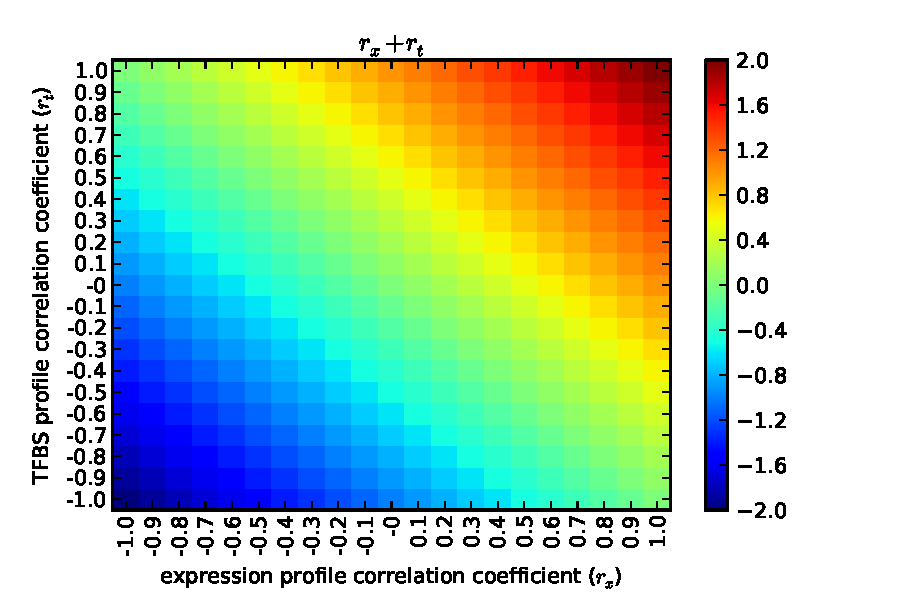
\includegraphics[width=.9\linewidth]{figures/figs/thesis-xprn-tfbs.pdf}
    \caption{}
    \label{fig:ptci-space-a}
  \end{subfigure}%

  

  \begin{subfigure}[b]{.9\linewidth}
    \centering

    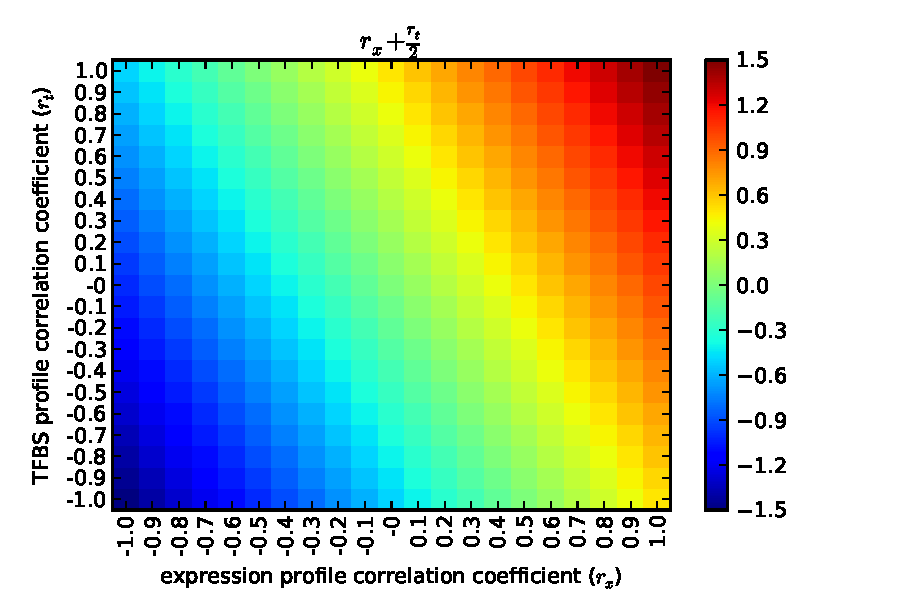
\includegraphics[width=.9\linewidth]{figures/figs/thesis-xprn-scaled-tfbs.pdf}
    \caption{}
    \label{fig:ptci-space-b}
  \end{subfigure}

\caption[Exploring the parameter space of the expression and TFBS components of the PTCI]{\sf \textbf{Exploring the parameter space of the expression and TFBS components of the PTCI:} \\
\textbf{(A)} The expression and \gls{TFBS} profile correlations each carry the same weight.  TFBS data is not strictly empirical, and position weight matrix models inherently are prone to produce false positive predictions. Here, each correlation-type exerts equal influence on the final score assigned to the ortholog relationship.  \textbf{(B)} The TFBS profile correlation is penalized due to the non-empirical nature and expected false positive information it contains. In this form, TFBS profile data contributes to the final score only 50\% as much as expression data.}
\label{fig:ptci-space}
\end{figure}